\documentclass[tikz,border=6pt]{standalone}
\usepackage{amsmath,amssymb,mathtools,physics,bm,nicefrac,wasysym}
\usepackage{xcolor}

\definecolor{colone}{RGB}{180,60,60}
\definecolor{coltwo}{RGB}{60,110,180}
\definecolor{colthree}{RGB}{60,140,80}

\definecolor{accent}{HTML}{A13D2C}
\definecolor{accent2}{HTML}{2B5F6B}
\definecolor{muted}{HTML}{5A564F}
\definecolor{panel}{HTML}{F8F6F0}
\definecolor{linecol}{HTML}{D8D2C4}
\definecolor{ink}{HTML}{1E1C1A}
\definecolor{astroblue}{HTML}{1B4F72}
\definecolor{astrodark}{HTML}{17202A}
\definecolor{sunyellow}{HTML}{E8A33D}

\usetikzlibrary{calc,arrows.meta,positioning,decorations.pathreplacing,decorations.markings,angles,quotes,shapes.geometric}
\usepackage{tikz-3dplot}

\newcommand{\vecr}{\vec r}
\newcommand{\vecL}{\vec L}
\newcommand{\vecA}{\vec A}
\newcommand{\vecf}{\vec f}
\newcommand{\vecF}{\vec F}
\newcommand{\vecp}{\vec p}
\newcommand{\avg}[1]{\left\langle #1\right\rangle}
\newcommand{\vecx}{\vec x}
\newcommand{\hatn}{\hat n}
\newcommand{\rhat}{\hat r}
\newcommand{\phihat}{\hat\phi}
\newcommand{\thetahat}{\hat\theta}
\newcommand{\note}[1]{\textcolor{blue!60!black}{\textit{[#1]}}}

% Astronomical acronyms
\newcommand{\LST}{\mathrm{LST}}
\newcommand{\GST}{\mathrm{GST}}
\newcommand{\GMST}{\mathrm{GMST}}
\newcommand{\GAST}{\mathrm{GAST}}
\newcommand{\LMST}{\mathrm{LMST}}
\newcommand{\LAST}{\mathrm{LAST}}
\newcommand{\UT}{\mathrm{UT}}
\newcommand{\UTC}{\mathrm{UTC}}
\newcommand{\TAI}{\mathrm{TAI}}
\newcommand{\TT}{\mathrm{TT}}
\newcommand{\TDB}{\mathrm{TDB}}
\newcommand{\JD}{\mathrm{JD}}
\newcommand{\MJD}{\mathrm{MJD}}
\newcommand{\EoT}{\mathrm{EoT}}
\newcommand{\SNR}{\mathrm{SNR}}
\newcommand{\RON}{\mathrm{RON}}

% Helper commands for specific diagrams
\newcommand{\midlinelabel}[3]{
    \node (midlabel) at ($ (#1)!.5!(#2) $) {#3};
    \draw[stealth-] (#1) --  (midlabel);
    \draw[-stealth] (midlabel) -- (#2);
}
\newcommand{\midlinelabell}[3]{
    \node[fill = white, inner sep = 0.2pt, outer sep=3pt] (midlabel) at ($ (#1)!.5!(#2) $) {#3};
    \draw[stealth-] (#1) --  (midlabel);
    \draw[-stealth] (midlabel) -- (#2);
}
\newcommand{\midlinelabelll}[3]{
    \node[fill = white, inner sep = 0.2pt, outer sep=3pt,scale=0.6] (midlabel) at ($ (#1)!.5!(#2) $) {#3};
    \draw[stealth-] (#1) --  (midlabel);
    \draw[-stealth] (midlabel) -- (#2);
}



\begin{document}
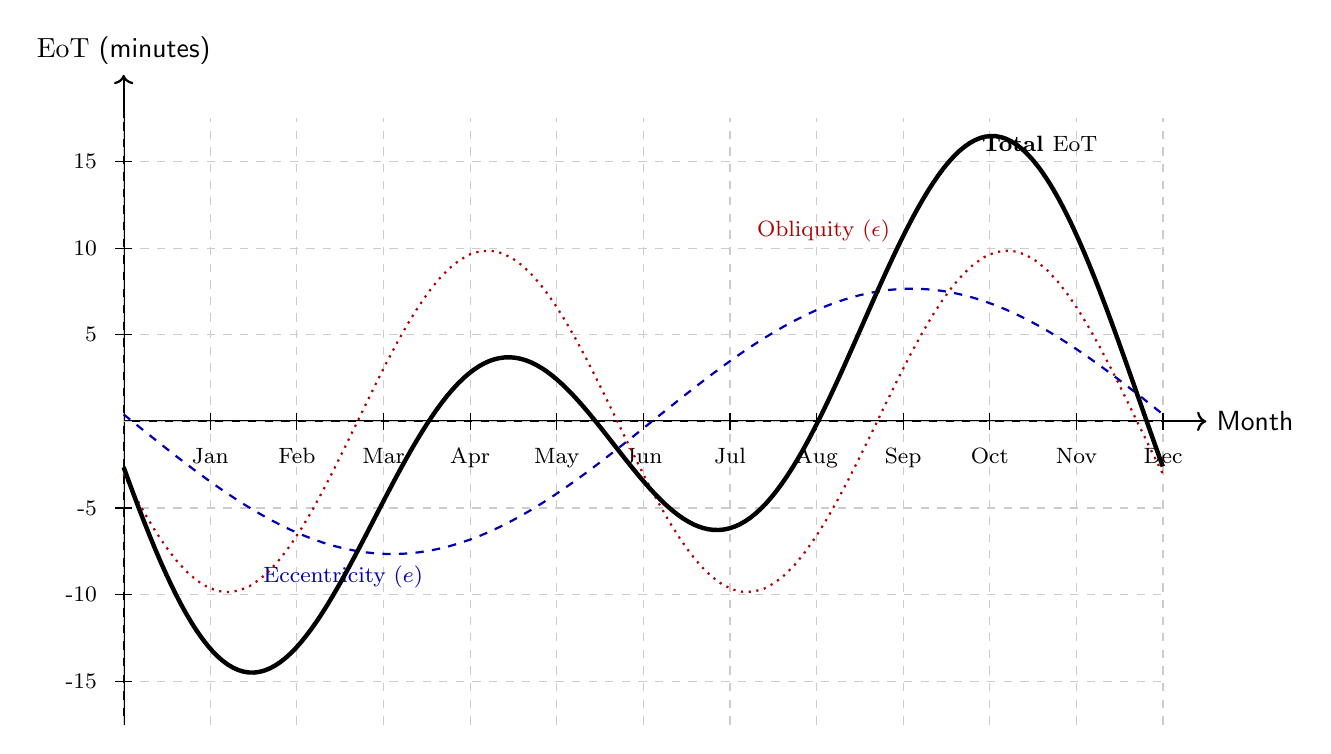
\begin{tikzpicture}[scale=1.1, font=\sffamily]
		\draw[->, thick] (0,0) -- (12.5,0) node[right] {Month};
		\draw[->, thick] (0,-3.5) -- (0,4.0) node[above] {$\EoT$ (minutes)};
		\draw[dashed, gray!40] (0,0) grid[xstep=1, ystep=1] (12,3.5);
		\draw[dashed, gray!40] (0,0) grid[xstep=1, ystep=1] (12,-3.5);
		
		% Ticks
		\foreach \x/\m in {1/Jan, 2/Feb, 3/Mar, 4/Apr, 5/May, 6/Jun, 7/Jul, 8/Aug, 9/Sep, 10/Oct, 11/Nov, 12/Dec} {
			\draw (\x, 0.1) -- (\x, -0.1) node[below=3pt, font=\footnotesize] {\m};
		}
		\foreach \y in {-15, -10, -5, 5, 10, 15} {
			\draw (0.1, \y*0.2) -- (-0.1, \y*0.2) node[left=3pt, font=\footnotesize] {\y};
		}
		
		% Component curves
		\draw[blue!70!black, thick, dashed, domain=0:12, samples=100] 
			plot (\x, {-7.66*sin(360*(\x-0.1)/12)*0.2});
		\node[blue!70!black, font=\footnotesize, right] at (1.5, -1.8) {Eccentricity ($e$)};
		
		\draw[red!70!black, thick, dotted, domain=0:12, samples=100] 
			plot (\x, {9.86*sin(720*(\x-2.7)/12)*0.2});
		\node[red!70!black, font=\footnotesize, right] at (7.2, 2.2) {Obliquity ($\epsilon$)};
		
		% Total curve
		\draw[black, ultra thick, domain=0:12, samples=200] 
			plot (\x, {(-7.66*sin(360*(\x-0.1)/12) + 9.86*sin(720*(\x-2.7)/12))*0.2});
		\node[black, font=\bfseries\footnotesize, right] at (9.8, 3.2) {Total $\EoT$};
	\end{tikzpicture}
\end{document}
